% !TEX program = xelatex
\documentclass[aspectratio=169, 11pt]{beamer}

\usetheme{metropolis}
\usepackage{appendixnumberbeamer}
\usepackage{array}
\usepackage{booktabs}
\usepackage{amsmath, amssymb}
\usepackage{graphicx}
\usepackage{tikz}
\usetikzlibrary{arrows.meta, positioning, patterns}
\usepackage{pgfplots}
\pgfplotsset{compat=1.18}

% Light theme — single accent color, no dark overrides
\definecolor{accent}{HTML}{A43F2A}
\setbeamercolor{progress bar}{fg=accent}
\setbeamercolor{alerted text}{fg=accent}
\setbeamercolor{frametitle}{bg=white, fg=black}

\setbeamerfont{frametitle}{size=\normalsize, series=\bfseries}

\title{An\'alisis de soluciones existentes}
\subtitle{Context Rot en LLMs: revisi\'on de literatura}
\author{Tom\'as Pablo Korenblit}
\date{Mayo 2026}
\institute{Licenciatura en Ciencia de Datos $\cdot$ Ciencia de Datos $\cdot$ 1C2026\\
Docentes: Rodrigo D\'iaz, Agust\'in Moro, Florencia Pi\~neyr\'ua}

\begin{document}

\maketitle

\begin{frame}{Delimitaci\'on del problema}

\textbf{Context Rot:} los LLM pierden adherencia a las instrucciones a medida que la conversaci\'on crece.

\end{frame}

\begin{frame}{La explosi\'on de la investigaci\'on en IA}

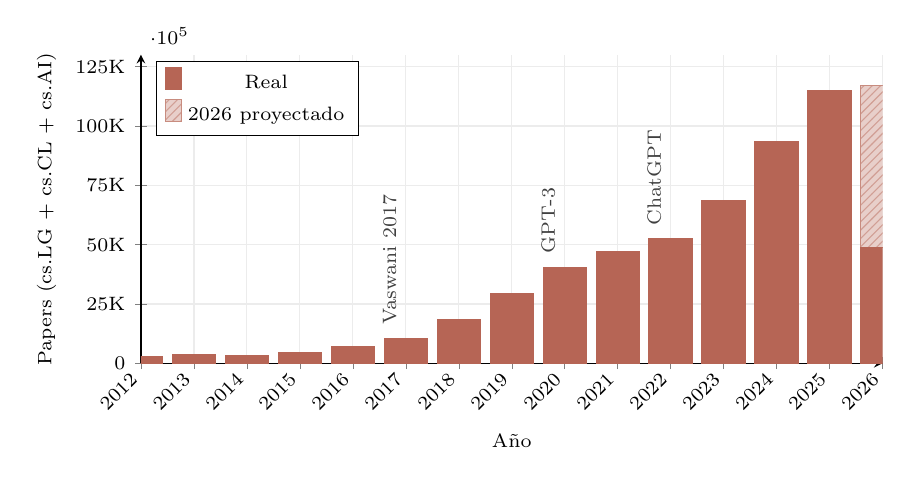
\begin{tikzpicture}
\begin{axis}[
    ybar stacked,
    width=11cm, height=5.5cm,
    bar width=0.55cm,
    xlabel={A\~no},
    ylabel={Papers (cs.LG + cs.CL + cs.AI)},
    xtick=data,
    xticklabels={2012,2013,2014,2015,2016,2017,2018,2019,2020,2021,2022,2023,2024,2025,2026},
    x tick label style={font=\scriptsize, rotate=45, anchor=east},
    y tick label style={font=\scriptsize},
    label style={font=\scriptsize},
    ymin=0, ymax=130000,
    ytick={0,25000,50000,75000,100000,125000},
    yticklabels={0,25K,50K,75K,100K,125K},
    grid=major, grid style={gray!15},
    axis lines=left,
    legend style={at={(0.02,0.98)}, anchor=north west, font=\scriptsize},
]
% Real data (solid)
\addplot[fill=accent!80, draw=accent!80] coordinates {
    (1,2699)(2,3471)(3,3323)(4,4439)(5,7213)(6,10467)
    (7,18508)(8,29445)(9,40431)(10,47138)(11,52498)
    (12,68478)(13,93511)(14,114891)(15,48770)
};
% Projected 2026 (hatched)
\addplot[fill=accent!25, draw=accent!60, postaction={pattern=north east lines, pattern color=accent!50}] coordinates {
    (1,0)(2,0)(3,0)(4,0)(5,0)(6,0)(7,0)(8,0)(9,0)
    (10,0)(11,0)(12,0)(13,0)(14,0)(15,68230)
};
\legend{Real, 2026 proyectado}

% Annotations
\node[font=\scriptsize, rotate=90, anchor=south west, text=darkgray]
    at (axis cs:6,10467) {\,Vaswani 2017};
\node[font=\scriptsize, rotate=90, anchor=south west, text=darkgray]
    at (axis cs:9,40431) {\,GPT-3};
\node[font=\scriptsize, rotate=90, anchor=south west, text=darkgray]
    at (axis cs:11,52498) {\,ChatGPT};
\end{axis}
\end{tikzpicture}

\vspace{-0.3em}
{\footnotesize Fuente: API arXiv, mayo 2026.}

\end{frame}

\begin{frame}{C\'omo funciona un LLM}

\begin{columns}[T]
\begin{column}{0.55\textwidth}
Un LLM predice el pr\'oximo token, dado todo el contexto anterior.
Para eso usa un mecanismo de \textbf{atenci\'on}: decide a qu\'e partes del contexto darle m\'as peso al generar cada token.

\vspace{0.8em}

La atenci\'on es un \textbf{recurso finito}. Se reparte entre todos los tokens del contexto.

\vspace{0.8em}

Las instrucciones del system prompt compiten por atenci\'on con todo lo que crece despu\'es.
\end{column}

\begin{column}{0.42\textwidth}
\renewcommand{\arraystretch}{1.4}
\begin{tabular}{@{} l r @{}}
\toprule
\textbf{A\~no} & \textbf{Tokens} \\
\midrule
2023 & 16K \\
2024 & 128--200K \\
2025 & 200K \\
2026 & \alert{\textbf{1M}} \\
\bottomrule
\end{tabular}

\vspace{0.6em}
\footnotesize
1M tokens $\approx$ 2.000 p\'aginas.
\end{column}
\end{columns}

\end{frame}

\begin{frame}{Trayectoria de la literatura}

\vspace{0.3em}

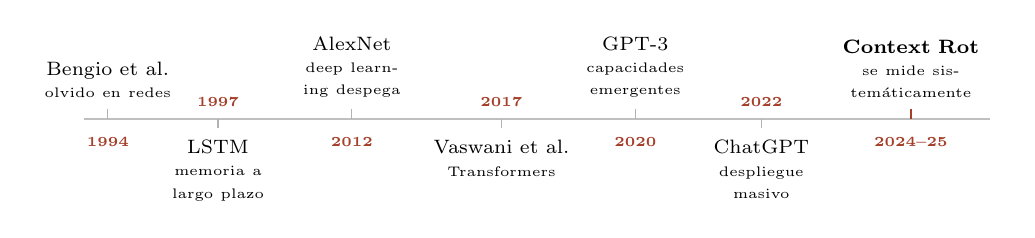
\begin{tikzpicture}[every node/.style={font=\scriptsize}]

% Timeline base
\draw[thick, gray!50] (0,0) -- (11.5,0);

% Hitos: x position, year, label (above=1/below=-1), text
% 1994 — above
\draw[gray!60] (0.3,0) -- (0.3,0.12);
\node[font=\tiny\bfseries, text=accent] at (0.3,-0.3) {1994};
\node[align=center, anchor=south, text width=1.8cm] at (0.3,0.15) {
    Bengio et al.\\{\tiny olvido en redes}
};

% 1997 — below
\draw[gray!60] (1.7,0) -- (1.7,-0.12);
\node[font=\tiny\bfseries, text=accent] at (1.7,0.22) {1997};
\node[align=center, anchor=north, text width=1.8cm] at (1.7,-0.15) {
    LSTM\\{\tiny memoria a largo plazo}
};

% 2012 — above
\draw[gray!60] (3.4,0) -- (3.4,0.12);
\node[font=\tiny\bfseries, text=accent] at (3.4,-0.3) {2012};
\node[align=center, anchor=south, text width=2cm] at (3.4,0.15) {
    AlexNet\\{\tiny deep learning despega}
};

% 2017 — below
\draw[gray!60] (5.3,0) -- (5.3,-0.12);
\node[font=\tiny\bfseries, text=accent] at (5.3,0.22) {2017};
\node[align=center, anchor=north, text width=2cm] at (5.3,-0.15) {
    Vaswani et al.\\{\tiny Transformers}
};

% 2020 — above
\draw[gray!60] (7.0,0) -- (7.0,0.12);
\node[font=\tiny\bfseries, text=accent] at (7.0,-0.3) {2020};
\node[align=center, anchor=south, text width=1.8cm] at (7.0,0.15) {
    GPT-3\\{\tiny capacidades emergentes}
};

% 2022 — below
\draw[gray!60] (8.6,0) -- (8.6,-0.12);
\node[font=\tiny\bfseries, text=accent] at (8.6,0.22) {2022};
\node[align=center, anchor=north, text width=1.8cm] at (8.6,-0.15) {
    ChatGPT\\{\tiny despliegue masivo}
};

% 2024-25 — above
\draw[accent, thick] (10.5,0) -- (10.5,0.12);
\node[font=\tiny\bfseries, text=accent] at (10.5,-0.3) {2024--25};
\node[align=center, anchor=south, text width=2.2cm] at (10.5,0.15) {
    \textbf{Context Rot}\\{\tiny se mide sistem\'aticamente}
};

\end{tikzpicture}

\vspace{0.8em}

\footnotesize
El problema del olvido existe desde 1994. Los Transformers lo convierten en otro tipo de olvido.\\
Reci\'en en 2024--2025 el campo empieza a estudiarlo sistem\'aticamente en conversaciones largas.

\end{frame}

% ─── CONTEXTO HISTÓRICO EXPANDIDO ───────────────────────────────────────────

\begin{frame}{La era pre-Transformers (1994--2016)}

\begin{columns}[T]
\begin{column}{0.48\textwidth}
\textbf{Bengio, Simard \& Frasconi (1994)}

\vspace{0.2em}
\textit{\scriptsize Learning Long-Term Dependencies with Gradient Descent is Difficult} \\ {\scriptsize IEEE Trans.\ Neural Networks}

\vspace{0.4em}
\footnotesize
Demostraron matem\'aticamente que las redes recurrentes vanilla \alert{no pueden} aprender dependencias largas: los gradientes se desvanecen o explotan al propagarse hacia atr\'as.

\vspace{0.4em}
El olvido en redes neuronales queda formalmente demostrado.
\end{column}

\begin{column}{0.48\textwidth}
\textbf{Hochreiter \& Schmidhuber (1997)}

\vspace{0.2em}
\textit{\scriptsize Long Short-Term Memory} \\ {\scriptsize Neural Computation}

\vspace{0.4em}
\footnotesize
Primera soluci\'on al problema de Bengio. Compuertas (\emph{input}, \emph{forget}, \emph{output}) que regulan qu\'e informaci\'on se mantiene a trav\'es del tiempo.

\vspace{0.4em}
Domin\'o NLP durante 20 a\~nos.
\end{column}
\end{columns}

\vspace{1.5em}

\begin{center}
\footnotesize
\emph{La memoria expl\'icita resuelve el olvido, pero la arquitectura es secuencial y dif\'icil de escalar.}
\end{center}

\end{frame}

\begin{frame}{La era Transformers (2017--2022)}

\begin{columns}[T]
\begin{column}{0.31\textwidth}
\textbf{Vaswani et al.\ (2017)}

\vspace{0.2em}
\textit{\scriptsize Attention Is All You Need} \\ {\scriptsize NeurIPS}

\vspace{0.4em}
\footnotesize
Reemplazan la recurrencia por atenci\'on pura. Permite paralelizar y escalar.

\vspace{0.4em}
\alert{Base de todos los LLMs modernos.}
\end{column}

\begin{column}{0.31\textwidth}
\textbf{Brown et al.\ (2020)}

\vspace{0.2em}
\textit{\scriptsize Language Models are Few-Shot Learners} \\ {\scriptsize NeurIPS}

\vspace{0.4em}
\footnotesize
GPT-3, 175B par\'ametros. Comportamiento \emph{emergente}: in-context learning, seguir instrucciones, razonar.

\vspace{0.4em}
\alert{La escala demuestra capacidades nuevas.}
\end{column}

\begin{column}{0.31\textwidth}
\textbf{Ouyang et al.\ (2022)}

\vspace{0.2em}
\textit{\scriptsize Training Language Models to Follow Instructions with Human Feedback} \\ {\scriptsize NeurIPS / InstructGPT}

\vspace{0.4em}
\footnotesize
RLHF aplicado a GPT-3. La base t\'ecnica de ChatGPT (nov.\ 2022).

\vspace{0.4em}
\alert{Los LLMs salen del laboratorio.}
\end{column}
\end{columns}

\end{frame}

\begin{frame}{Por qu\'e los Transformers no resolvieron el olvido}

\begin{columns}[T]
\begin{column}{0.48\textwidth}
\textbf{LSTM}

\vspace{0.3em}
\footnotesize
Memoria expl\'icita con compuertas. Mantiene informaci\'on a largo plazo \emph{por dise\~no}.

\vspace{0.4em}

\textbf{Costo:} arquitectura secuencial. No escala bien.
\end{column}

\begin{column}{0.48\textwidth}
\textbf{Transformer}

\vspace{0.3em}
\footnotesize
Atenci\'on global sobre el contexto. Paraleliza y escala a millones de tokens.

\vspace{0.4em}

\textbf{Costo:} la atenci\'on es un \emph{recurso finito} que se reparte entre todos los tokens. No hay memoria privilegiada.
\end{column}
\end{columns}

\vspace{1em}

\begin{alertblock}{}
\footnotesize
Los Transformers escalaron sacrificando memoria expl\'icita. La atenci\'on global se diluye cuando el contexto crece. \textbf{Eso es Context Rot.}
\end{alertblock}

\end{frame}

% ─── MEDICIÓN ────────────────────────────────────────────────────────────────

\begin{frame}{Laban et al.\ (2025)}

\textit{LLMs Get Lost in Multi-Turn Conversation} (preprint arXiv, Microsoft + Salesforce)

\vspace{0.6em}

\begin{columns}[T]
\begin{column}{0.48\textwidth}
\textbf{Qu\'e hicieron}

\vspace{0.3em}
\footnotesize
Compararon el mismo modelo en dos escenarios: \emph{single-turn fully-specified} (toda la informaci\'on de una sola vez) vs \emph{multi-turn sharded} (la misma tarea fragmentada en turnos). 15 modelos de 8 familias, 6 tareas de generaci\'on.
\end{column}

\begin{column}{0.48\textwidth}
\textbf{Qu\'e encontraron}

\vspace{0.3em}
\footnotesize
Ca\'ida promedio del \alert{\textbf{39\%}} entre single-turn y multi-turn. Pasa en \alert{los 15 modelos}.

\vspace{0.6em}

Detalle: la capacidad (\emph{aptitude}) baja solo $\sim$16\%. La \alert{varianza sube 112\%}. La aptitud cae poco; lo que explota es la inestabilidad.
\end{column}
\end{columns}

\vspace{0.6em}

\begin{alertblock}{La brecha que importa}
\footnotesize
\textbf{Limitaci\'on (autores):} simulaci\'on autom\'atica, solo ingl\'es. \\
\textbf{Para mi trabajo:} \alert{no desagregan por tipo de instrucci\'on}. Este es el hueco que el proyecto final va a llenar.
\end{alertblock}

\end{frame}

% ─────────────────────────────────────────────────────────────────────────────

\begin{frame}{He et al.\ (2024), Meta}

\textit{Multi-IF: Benchmarking LLMs on Multi-turn and Multilingual Instruction Following}

\vspace{0.6em}

\begin{columns}[T]
\begin{column}{0.48\textwidth}
\textbf{Qu\'e hicieron}

\vspace{0.3em}
\footnotesize
En cada turno agregan una instrucci\'on nueva al contexto (sin remover las anteriores). 14 modelos, 8 idiomas, 4.501 conversaciones de 3 turnos.

\vspace{0.5em}

Definen \alert{Instruction Forgetting Ratio (IFR)}: \% de instrucciones que el modelo cumpli\'o antes pero deja de cumplir en turnos posteriores.
\end{column}

\begin{column}{0.48\textwidth}
\textbf{Qu\'e encontraron}

\vspace{0.3em}
\footnotesize
o1-preview: \alert{\textbf{87{,}7\% $\to$ 70{,}7\%}} de turno 1 a turno 3 (promedio sobre 8 idiomas).

\vspace{0.6em}

Las instrucciones est\'an en el contexto, no desaparecen. Pero el modelo deja de aplicarlas a medida que se agregan nuevas.

\vspace{0.6em}

\textbf{Limitaci\'on (autores):} las conversaciones reales son de 10+ turnos. Multi-IF solo cubre 3.
\end{column}
\end{columns}

\end{frame}

% ─── MECANISMO ────────────────────────────────────────────────────────────────

\begin{frame}{Liu et al.\ (2024)}

\textit{Lost in the Middle: How Language Models Use Long Contexts}, TACL

\vspace{0.4em}

\begin{columns}[T]
\begin{column}{0.52\textwidth}
\textbf{Qu\'e hicieron}

\vspace{0.3em}
\footnotesize
Dos tareas: QA multi-documento y recuperaci\'on clave-valor sint\'etica. En ambas, el item relevante se ubic\'o en distintas posiciones del contexto. 7 modelos.

\vspace{0.4em}

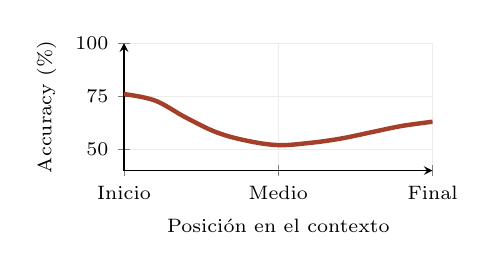
\begin{tikzpicture}
\begin{axis}[
    width=5.5cm, height=3.2cm,
    xlabel={Posici\'on en el contexto},
    ylabel={Accuracy (\%)},
    xmin=0, xmax=10, ymin=40, ymax=100,
    xtick={0, 5, 10}, xticklabels={Inicio, Medio, Final},
    ytick={50, 75, 100},
    grid=major, grid style={gray!15},
    axis lines=left,
    label style={font=\scriptsize},
    tick label style={font=\scriptsize},
]
\addplot[color=accent, ultra thick, smooth, tension=0.6]
    coordinates {(0,76)(1,73)(2,65)(3,58)(4,54)(5,52)
                 (6,53)(7,55)(8,58)(9,61)(10,63)};
\end{axis}
\end{tikzpicture}
\end{column}

\begin{column}{0.44\textwidth}
\textbf{Qu\'e encontraron}

\vspace{0.3em}
\footnotesize
\alert{Curva U asim\'etrica}: el inicio se retiene mejor que el final, el medio peor que ambos. En multi-doc QA con 20 docs, GPT-3.5 cae de \textasciitilde75\% (inicio) a \textasciitilde52\% (medio).

\vspace{0.6em}

El paper documenta el efecto pero \alert{no mide atenci\'on}. La conexi\'on con system prompts en posici\'on 0 es extrapolaci\'on m\'ia.

\vspace{0.6em}

\textbf{Limitaci\'on (autores):} tareas de recuperaci\'on en ingl\'es; ni instrucciones ni casos realistas.
\end{column}
\end{columns}

\end{frame}

% ─────────────────────────────────────────────────────────────────────────────

\begin{frame}{Mu et al.\ (2025)}

\textit{A Closer Look at System Prompt Robustness} (UC Berkeley)

\vspace{0.6em}

\begin{columns}[T]
\begin{column}{0.48\textwidth}
\textbf{Qu\'e hicieron}

\vspace{0.3em}
\footnotesize
Prueba de estr\'es ``Monkey Island'': partieron de un system prompt real y agregaron de \alert{1 a 20 guardrails}. Modelo y tarea fijos. 5 modelos v\'ia API (familia GPT-4o, o3-mini, DeepSeek V3/R1).

\vspace{0.6em}

Dato de contexto: en prompts reales del GPT Store hay un \alert{promedio de 5.1 guardrails} por prompt. La producci\'on ya opera cerca de la zona problem\'atica.
\end{column}

\begin{column}{0.48\textwidth}
\textbf{Qu\'e encontraron}

\vspace{0.3em}
\footnotesize
Al pasar de 1 a 20 guardrails, la adherencia a cada uno \alert{se aproxima a 0\%} de forma uniforme entre modelos.

\vspace{0.6em}

\textbf{Saturaci\'on:} las instrucciones compiten entre s\'i. Mecanismo distinto al de Liu: ac\'a el problema es la \alert{cantidad}, no la posici\'on.

\vspace{0.6em}

\textbf{Inferencia m\'ia:} si m\'as reglas degradan la adherencia, repetir el prompt entero (que multiplica reglas en contexto) probablemente la degrade tambi\'en.
\end{column}
\end{columns}

\end{frame}

% ─── AI SAFETY ────────────────────────────────────────────────────────────────

\begin{frame}{Implicaciones de seguridad}

\begin{columns}[T]
\begin{column}{0.48\textwidth}
\textbf{Anil et al.\ (2024, Anthropic)}

\vspace{0.3em}
\footnotesize
\textit{Many-shot Jailbreaking}

\vspace{0.5em}

Evidencia emp\'irica: la tasa de jailbreak aumenta de forma sistem\'atica con el n\'umero de ejemplos previos en el contexto. M\'as largo $\Rightarrow$ m\'as vulnerable.
\end{column}

\begin{column}{0.48\textwidth}
\textbf{Rivasseau (2025)}

\vspace{0.3em}
\footnotesize
\textit{LLM Reinforcement in Context}

\vspace{0.5em}

Formalizaci\'on te\'orica del problema: el ratio de tokens del system prompt sobre el contexto total tiende a 0 con el largo. Propone insertar ``interrupciones'' peri\'odicas como mitigaci\'on (sin evaluaci\'on emp\'irica).
\end{column}
\end{columns}

\vspace{0.8em}

\begin{alertblock}{}
\footnotesize
Los guardrails son instrucciones como cualquier otra. Si decaen, el sistema falla silenciosamente: sin alarma, sin error visible.
\end{alertblock}

\end{frame}

% ─── MITIGACIONES ────────────────────────────────────────────────────────────

\begin{frame}{Repetir el prompt (pr\'actica com\'un)}

\textit{Sin paper formal. Es la pr\'actica m\'as com\'un en sistemas en producci\'on.}

\vspace{0.8em}

\begin{columns}[T]
\begin{column}{0.48\textwidth}
\textbf{Qu\'e se hace}

\vspace{0.3em}
\footnotesize
Re-inyectar el system prompt completo al comienzo de cada turno. Todas las instrucciones, siempre, sin distinci\'on.
\end{column}

\begin{column}{0.48\textwidth}
\textbf{Lo que s\'i se sabe}

\vspace{0.3em}
\footnotesize
Costo: $N\times$ tokens por conversaci\'on.

\vspace{0.6em}

Mu et al.\ (2025): con m\'as reglas en el prompt, la adherencia a cada una baja. Repetir todo puede \alert{empeorar} la situaci\'on.

\vspace{0.6em}

\textbf{Limitaci\'on de la literatura:} nadie mide cu\'antos sistemas la usan ni cu\'anto ayuda o perjudica en conversaciones largas reales.
\end{column}
\end{columns}

\end{frame}

\begin{frame}{Wallace et al.\ (2024), OpenAI}

\textit{The Instruction Hierarchy: Training LLMs to Prioritize Privileged Instructions}

\vspace{0.6em}

\begin{columns}[T]
\begin{column}{0.48\textwidth}
\textbf{Qu\'e hicieron}

\vspace{0.3em}
\footnotesize
Entrenaron GPT-3.5 Turbo (SFT + RLHF) para priorizar instrucciones seg\'un origen:

\vspace{0.3em}
\textbf{system} $>$ \textbf{usuario} $>$ \textbf{multimodal} $>$ \textbf{tool outputs}.

\vspace{0.5em}
La jerarqu\'ia se aprende en el entrenamiento, no se impone en contexto.
\end{column}

\begin{column}{0.48\textwidth}
\textbf{Qu\'e encontraron}

\vspace{0.3em}
\footnotesize
+63\% robustez frente a extracci\'on del system prompt. +30\% frente a jailbreaks.

\vspace{0.6em}

\textbf{Limitaci\'on (autores):} regresiones en over-refusal — a veces rechaza consultas benignas.

\vspace{0.5em}

\textbf{Mi extensi\'on:} la jerarqu\'ia ordena \emph{roles}, no instrucciones individuales. Dentro de un mismo rol, no aborda el decay temporal.
\end{column}
\end{columns}

\end{frame}

\begin{frame}{Leviathan et al.\ (2025), Google Research}

\textit{Prompt Repetition Improves Non-Reasoning LLMs}

\vspace{0.6em}

\begin{columns}[T]
\begin{column}{0.48\textwidth}
\textbf{Qu\'e hicieron}

\vspace{0.3em}
\footnotesize
Duplican el prompt entero back-to-back: \texttt{<QUERY><QUERY>}. 7 modelos (Gemini, GPT-4o, Claude, DeepSeek), 7 benchmarks.

\vspace{0.5em}

Mecanismo propuesto: la atenci\'on causal impide que tokens iniciales atiendan a posteriores. Repetir permite una ``segunda pasada''.
\end{column}

\begin{column}{0.48\textwidth}
\textbf{Qu\'e encontraron}

\vspace{0.3em}
\footnotesize
\alert{47 victorias y 0 derrotas} sobre 70 combinaciones, en modelos no-razonadores. En modelos con chain-of-thought el efecto es nulo o leve.

\vspace{0.6em}

\textbf{Limitaci\'on:} duplica los tokens de \emph{entrada} (no la salida ni la latencia). Sigue siendo uniforme: duplica todo el prompt por igual, sin priorizar.
\end{column}
\end{columns}

\end{frame}

\begin{frame}{Dongre et al.\ (2025)}

\textit{Drift No More? Context Equilibria in Multi-Turn LLM Interactions} (Adobe Research + UIUC, preprint arXiv)

\vspace{0.6em}

\begin{columns}[T]
\begin{column}{0.48\textwidth}
\textbf{Qu\'e hicieron}

\vspace{0.3em}
\footnotesize
Inyectaron recordatorios del objetivo en \alert{turnos fijos $t=4$ y $t=7$} sobre conversaciones de 10 turnos ($\tau$-Bench). Tres modelos como simuladores de usuario (Llama-3.1-8B, 70B, Qwen 2).

\vspace{0.4em}

Formalizaron el drift como divergencia KL respecto a una pol\'itica de referencia (GPT-4.1).
\end{column}

\begin{column}{0.48\textwidth}
\textbf{Qu\'e encontraron}

\vspace{0.3em}
\footnotesize
El drift se \alert{estabiliza en un equilibrio finito}; no crece sin techo. Los recordatorios bajan ese equilibrio (Llama-8B: 20,4 $\to$ 17,6).

\vspace{0.6em}

\textbf{Limitaci\'on:} calendario fijo, no adaptativo. No seleccionan qu\'e instrucci\'on reinyectar seg\'un historial de compliance.
\end{column}
\end{columns}

\end{frame}

\begin{frame}{Comparaci\'on de mitigaciones}

\renewcommand{\arraystretch}{1.5}
\begin{table}
\centering
\footnotesize
\begin{tabular}{@{} >{\raggedright\arraybackslash}p{2.8cm} >{\raggedright\arraybackslash}p{3.2cm} >{\raggedright\arraybackslash}p{1.9cm} >{\raggedright\arraybackslash}p{3.1cm} @{}}
\toprule
\textbf{M\'etodo} & \textbf{Idea} & \textbf{Costo} & \textbf{Limitaci\'on} \\
\midrule
Repetir prompt & Re-inyectar todo cada turno & $N\times$ input & Saturaci\'on (Mu) \\
Wallace (2024) & Jerarqu\'ia de roles en training & Cero & Est\'atica \\
Leviathan (2025) & \texttt{<Q><Q>} (duplicar) & $2\times$ input & Uniforme \\
Dongre (2025) & Reminders fijos & $\sim 1.2\times$ & No adaptativo \\
\bottomrule
\end{tabular}
\end{table}

\vspace{0.6em}

\begin{center}
\footnotesize
Cuatro estrategias, cuatro costos, cuatro l\'imites.\\
Todas \alert{\textbf{uniformes}} sobre el conjunto de instrucciones.
\end{center}

\end{frame}

% ─── MARCO + LO QUE FALTA ────────────────────────────────────────────────────

\begin{frame}{Marco te\'orico y lo que falta}

\begin{columns}[T]
\begin{column}{0.48\textwidth}
\textbf{Zhang, Yang \& Wang (2025)}

\vspace{0.3em}
\footnotesize
LLM peque\~nos (Llama-8B, Mistral-7B, Gemma-2B) se comportan como \emph{filtros bayesianos descontados} ($\gamma < 1$): el prior pierde peso frente a las observaciones recientes.

\vspace{0.5em}

El paper no habla de instrucciones; el puente con compliance es m\'io. \emph{Conecta con Laban: la varianza explota porque el posterior se vuelve inestable.}

\vspace{0.7em}

\textbf{Greenblatt et al.\ (ICML 2024)}: \emph{AI Control} en runtime. Marco complementario; los protocolos que proponen quedan expuestos si decae cualquier instrucci\'on en contexto.
\end{column}

\begin{column}{0.48\textwidth}
\begin{block}{El hueco que importa}
\footnotesize
\begin{itemize}
    \item \alert{Nadie midi\'o si el decay var\'ia seg\'un el tipo de instrucci\'on.} Sin eso, todo refuerzo selectivo es injustificado.
    \item Anthropic, OpenAI, Google y Meta no publicaron investigaci\'on primaria sobre Context Rot.
    \item Las mitigaciones son uniformes porque \emph{no tienen datos para discriminar}.
\end{itemize}
\end{block}
\end{column}
\end{columns}

\end{frame}

% ─── ORIENTACIÓN ─────────────────────────────────────────────────────────────

\begin{frame}{Orientaci\'on del proyecto final}

Antes de armar un BKT selectivo hab\'ia que verificar el supuesto: ¿realmente las instrucciones decaen distinto?

\vspace{0.8em}

\textbf{Estudio que hice:}
\begin{itemize}
    \item 28 conversaciones $\cdot$ 244 observaciones $\cdot$ 5 modelos
    \item Modelo log\'istico ordinal bayesiano, efectos jer\'arquicos por tipo de decisi\'on
    \item \textbf{Resultado:} $\sigma_\beta = 2{,}11$ (intervalo de credibilidad del 94\%: $[1{,}06,\ 3{,}28]$). La heterogeneidad existe.
\end{itemize}

\vspace{0.6em}

\textbf{Pr\'oximo paso:} armar el BKT con presupuesto fijo de tokens y compararlo contra refuerzo uniforme.

\vspace{0.8em}

\footnotesize\itshape
Trabajo sometido a JAIIO 55. Se anuncia a fines de mayo. No es resultado validado por pares todav\'ia.

\end{frame}

\appendix

\begin{frame}{Referencias}

\scriptsize
\begin{columns}[T]
\begin{column}{0.48\textwidth}
Bengio, Y., Simard \& Frasconi (1994). \emph{Learning Long-Term Dependencies with Gradient Descent is Difficult}. IEEE Trans.\ NN.\par\medskip
Hochreiter \& Schmidhuber (1997). \emph{Long Short-Term Memory}. Neural Computation.\par\medskip
Krizhevsky, Sutskever \& Hinton (2012). \emph{ImageNet Classification with Deep CNNs} (AlexNet). NeurIPS.\par\medskip
Vaswani et al.\ (2017). \emph{Attention Is All You Need}. NeurIPS.\par\medskip
Brown et al.\ (2020). \emph{Language Models are Few-Shot Learners} (GPT-3). NeurIPS.\par\medskip
Ouyang et al.\ (2022). \emph{Training LMs to Follow Instructions with HF} (InstructGPT). NeurIPS.\par\medskip
Anil, C.\ et al.\ (2024). \emph{Many-shot Jailbreaking}. Anthropic, NeurIPS.\par\medskip
Liu, N.\ F.\ et al.\ (2024). \emph{Lost in the Middle}. TACL.\par\medskip
He, B.\ et al.\ (2024). \emph{Multi-IF}. Meta.\par
\end{column}

\begin{column}{0.48\textwidth}
Wallace, E.\ et al.\ (2024). \emph{The Instruction Hierarchy}. OpenAI.\par\medskip
Greenblatt, R.\ et al.\ (2024). \emph{AI Control}. ICML.\par\medskip
Laban, P.\ et al.\ (2025). \emph{LLMs Get Lost in Multi-Turn Conversation}. arXiv preprint.\par\medskip
Mu, N.\ et al.\ (2025). \emph{A Closer Look at System Prompt Robustness}. UC Berkeley.\par\medskip
Zhang, Yang \& Wang (2025). \emph{LLMs as Discounted Bayesian Filters}.\par\medskip
Leviathan et al.\ (2025). \emph{Prompt Repetition Improves Non-Reasoning LLMs}. Google.\par\medskip
Dongre, V.\ et al.\ (2025). \emph{Drift No More?}. Adobe + UIUC, preprint arXiv.\par\medskip
Rivasseau, T.\ (2025). \emph{LLM Reinforcement in Context}. arXiv.\par\medskip
Chroma Research (2025). \emph{Context Rot}. Industria.\par
\end{column}
\end{columns}

\end{frame}

\end{document}
